\section{Related Work}

Previous work applying augmented reality to retail shopping has focused on how designers and system architects properly utilize this novel technology \cite{ahn2015supporting,kourouthanassis2007enhancing,olsson2013expected,spreer2012improving,stoyanova2015comparison,zhu2004personalized}.  \todo{DNS: Pull out a few of these citations into specific examples. E.g., "For example, Ahn et al. did something interesting. Olsson et al. did something else. These efforts highlight the importance of context provided by AR for consumer decision making. However, they don't do something that we do..."} Context-awareness is a useful affordance provided by augmented reality.  Designers find that this ability to visually associate digital content with products increases customer empowerment, user efficiency in gathering information, and system influence. \todo{cite source? DNS: Yes, please!} Other AR application domains focus on collaborative experiences and visualizations \cite{esser2016head,santos2016augmented,truong2013today}. \todo{DNS: Should add a note here on what specifically they tell us about this application}

\begin{marginfigure}
	\begin{minipage}{\marginparwidth}
		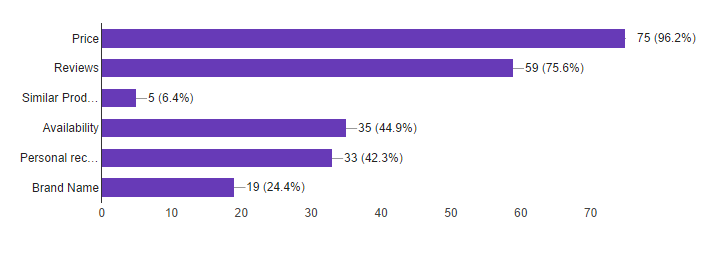
\includegraphics[width=0.9\columnwidth]{figures/ShoppingFactors}
		\caption{Phase One respondants identified price and reviews as the most critical factors in making their shopping decisions, while product comparisons---identified in later phases as ``highly useful''---were initially rated as least important. \textbf{DNS: Axis labels please!!! Turn into vertical chart s.t. it's legible as a margin fig. Also use full labels rather than ellipses. May have to reconstruct in powerpoint or inkscape}}
		\label{figures:ShoppingFactors}
	\end{minipage}
\end{marginfigure}

\todo[inline]{DNS: Do we have any insight into how current systems are designed? That may be a nice transition from conventional systems and this approach.}

Much of this previous work has focused on mobile augmented reality (MAR). However, MAR systems suffer from a number of limitations for retail shopping such as insufficient processing power, required use of hands and an intermediate screen, and a field of view constrained by screen size \cite{bimber2005spatial} \todo{DNS: Did a bit of refactoring here. Take a santiy check to make sure this is still saying the right thing.}  Head-mounted displays (HMDs) such as Microsoft's Hololens offer opportunities to overcome these limitations, and the ability to synchronize data with head movements may allow consumers passive access to visual information in context. In this work, we explore how systems might effectively leverage HMDs to provide product information in context for traditional retail environments. \todo{DNS: It might be the right call to just blend this with the next paragraph. }
%reaching the mainstream, head-mounted displays (HMD) are gaining attention as a potential platform for AR experiences.  U

Other work has introduced spatial augmented reality (SAR) systems and applications.  SAR applications employ ubiquitous computing to project context-aware digital content into the user's physical environment \cite{benko2015fovear,benko2014dyadic}.  Technical advantages of a SAR system include removing the need for users to wear or carry often cumbersome equipment and a non-restricted field of view.  \todo{DNS: yep, really might be good to blend with the previous paragraph and leave some space to talk about design since that is a contribution of the work} %Resolution could potentially improve, since computation and graphics processing hardware would not be constrained by form factor - a limitation for HMD which must not be too bulky to be worn on the user's head.  
However, one limitation of SAR systems is that they require a static, controlled environment to be used effectively due to the use of fixed displays. \todo{is there a source that supports this? From your notes it seems that "Spatial Augmented Reality Merging Real and Virtual Worlds" might}

In this paper, we take a user-centered design approach to testing how the theoretical grounding derived from this previous work on mobile and spatial augmented reality applies to HMD-based augmented reality. \todo{but this doesn't build on previous work. Maybe something like "We explore how a user-centered design approach might enable us to draw from existing experiences to craft new AR experiences"} We also examine how HMD-based AR may combine some of the benefits of these approaches while removing some of their limitations. Our work iterates on this approach in three distinct development phases: an open-ended survey, a low fidelity prototype, and a high fidelity prototype. \todo{DNS: Not attached to this sentence specifically, but some sort of transition to methodology is needed here}